
\documentclass[a4paper, 10pt, twocolumn]{article}

\usepackage[utf8]{inputenc}               
\usepackage[english]{babel}    
\usepackage{lipsum}
\usepackage{makecell}
\usepackage{graphicx}
\graphicspath{ {./images/} }

\begin{document}

\section{K-NN and /decision Trees}
Distances, $d(x^{(i)},x^{(q)})$ = \\
\begin{tabular}{ c c c }
	Manhattan & L1 & $\sum^{K}_{k=1}|x^{(i)}_{k} - x_{k}^{(q)}|$ \\ 
	Euclidean & L2 & $\sqrt{\sum^{K}_{k=1}(x^{(i)}_{k} - x_{k}^{(q)})^2}$  \\  
	Chebyshev & L$\infty$ & $\max^K_{k=1}|x^{(i)}_{k} - x_{k}^{(q)}|$    
\end{tabular} \\ \\ \\
Types = 
\begin{tabular}{ c c }
	Inverse & $\frac{1}{d(x^{(i)},x^{(q)})}$ \\ 
	Gaussian & $\frac{1}{\sqrt{2 \pi}}\exp(-\frac{d(x^{(i)},x^{(q)})^2}{2})$  \\     
\end{tabular} \\ \\ \\
Entropy = $H(X)$ =
\begin{tabular}{ c }
	$-\sum^K_k P(x_k) \log_2(P(x_k))$ \\
	$-\int_k f(x) \log_2(f(x))$
\end{tabular} \\ \\ \\
Information Gain = $\textrm{IG}(\textrm{dataset},\textrm{subsets})$\\ 
\begin{tabular} {c}
	$ = H(dataset) - \sum_{S \in \textrm{subsets}} \frac{|S|}{|\textrm{dataset}|H(S)}$ \\
	$|\textrm{dataset}| = \sum_{S \in \textrm{subsets}} |S|$
\end{tabular}
\section{Evaluation of Machine Learning Systems}
Confusion Matrix \\ \\
\begin{tabular} {| c | c | c |}
	\hline
 & \thead{Class 1 \\ Predicted} & \thead{Class 2 \\ Predicted} \\
 \hline
 \thead{Class 1 \\ Actual} &  \thead{\bf TP \\ True Positive} & \thead{\bf FN \\False Negative} \\
 \hline
 \thead{Class 2 \\ Actual} &  \thead{\bf FP \\ False Positive} & \thead{\bf TN \\ True Negative} \\
 \hline
\end{tabular} \\
Accuracy = $\frac{TP + TN}{TP + TN + FP + FN}$ \\ 
Precision = $\frac{TP}{TP + FP}$ \\
Recall = $\frac{TP}{TP + FN}$ \\
F-measure = $F_1 = 2\frac{Precision*Recall}{Precision + Recall}$\\
MSE = $\frac{1}{N} \sum^{N}_{i=1}(Y_i - \hat{Y}_i)^2$\\
Sample Error: \\$error_s(h) = \frac{1}{N} \sum_{x \in S} \delta (f(x),h(x))$\\
Confidence interval: \\ $error_s(h) \pm Z_N \sqrt{\frac{error_s(h)*(1-error_s(h))}{n}}$
\section{Neural Networks}
Activation Functions: \\ 
\begin{tabular}{c c c}
	Function & $g(z)$ & $g'(z)$ \\
	Sigmoid & $\frac{1}{1 + e^{-x}}$ & $g(z)(1-g(z))$ \\
	Tanh & $\frac{e^x  - e^{-x}}{e^x + e^{-x}}$ & $1-g(z)^2$ \\
	ReLU & \thead{$0$ for $x \leq 0 $ \\ $x$ for $x>0$} & \thead{$0$ for $x \leq 0 $ \\ $1$ for $x>0$} \\
	Softmax & $\frac{e^{Z_i}}{\sum_k e^{Z_k}}$ & $\frac{\delta L}{\delta z} = \frac{1}{N} (\hat y - y)$
\end{tabular} \\ \\
Back Propagation:\\
$\frac{\delta \textrm{Loss}}{\delta W} = \frac{\delta \textrm{Loss}}{\delta Z} \cdot \frac{\delta Z}{\delta W}$ \\
$\frac{\delta \textrm{Loss}}{\delta b} = \frac{\delta \textrm{Loss}}{\delta Z} \cdot \frac{\delta Z}{\delta b}$ \\
$\frac{\delta \textrm{Loss}}{\delta X} = \frac{\delta \textrm{Loss}}{\delta Z} \cdot \frac{\delta Z}{\delta X}$ \\
$\frac{\delta \textrm{Loss}}{\delta X} = \frac{\delta \textrm{Loss}}{\delta Z} \cdot W^T$ \\
$\frac{\delta \textrm{Loss}}{\delta W} = X^T \cdot \frac{\delta \textrm{Loss}}{\delta Z}$ \\
$\frac{\delta \textrm{Loss}}{\delta b} = 1^T \cdot \frac{\delta \textrm{Loss}}{\delta Z}$ \\
$\frac{\delta \textrm{Loss}}{\delta Z} = \frac{\delta \textrm{Loss}}{\delta A} \circ g'(Z)$ \\
where $A = g(Z)$ \\ \\ Regularisation \\
$L1: J(\theta) = \textit{Loss}(y,\hat y) + \lambda \sum_w w^2$ \\
$w \leftarrow w - \alpha(\frac{\delta \textit{Loss}}{\delta w} + 2 \lambda w)$ \\
$L2: J(\theta) = \textit{Loss}(y,\hat y) + \lambda \sum_w |w|$ \\
$w \leftarrow w - \alpha(\frac{\delta \textit{Loss}}{\delta w} + 2 \sin w)$ \\
Dropout: drop $50\%$ of Activation \\ \\
Data normalisation\\
Min-Max: $X' = a + \frac{(X -X_{min})(b-a)}{X_{max}-X_{min}}$ \\
Standardization: $X' = \frac{X-\mu}{\sigma }$
\section{Unsupervised Learning} 
K-means \\
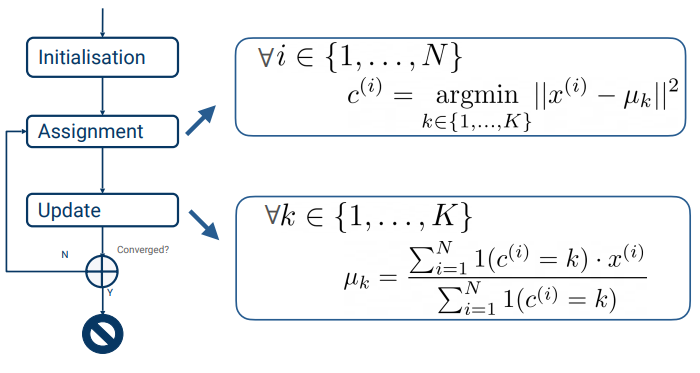
\includegraphics[scale=0.5]{k-means.png} \\
GMM-EM \\
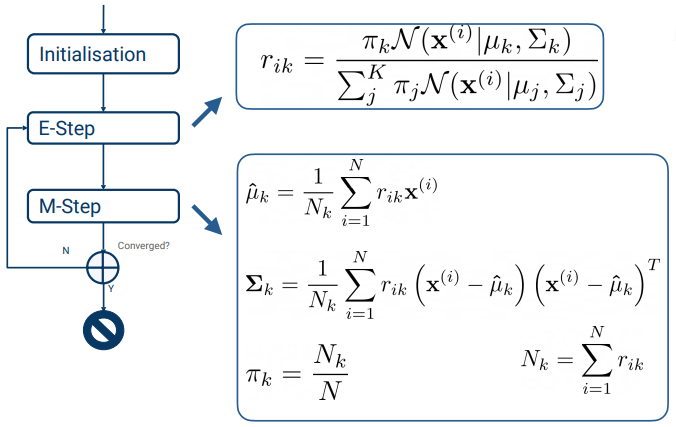
\includegraphics[scale=0.5]{GMM-EM.png} \\ \\
Mixture Models: \\$p(x) = \sum^K_{k=1} \pi_k p_k(x)$ \\
Gaussian Mixture models: \\$p(x|\theta) = \sum^K_{k=1} \pi_k \mathcal{N}(x|\mu_k, \sum_k)$
\section{Evolutionary Algorithms}

\section{General}
Overfitting
\begin{enumerate}
	\item high dimensionality $\rightarrow$  overfitting
	\item Stop for decision trees (Pruning, early stopping (max depth))
	\item General Solutions (more data, stop earlier and change complexity (use validation set to test))
	\item Neural networks (dropout/regularisation/normalisation)
\end{enumerate}
\end{document}